\documentclass[tikz, border=15pt]{standalone}
\usepackage{amsmath, amssymb}
% Added 'shadows' to the library list here!
\usetikzlibrary{positioning, arrows.meta, matrix, shapes.geometric, calc, shadows}

\begin{document}
	
	% Define the finite field macro
	\newcommand{\F}{\mathbb{F}}
	
	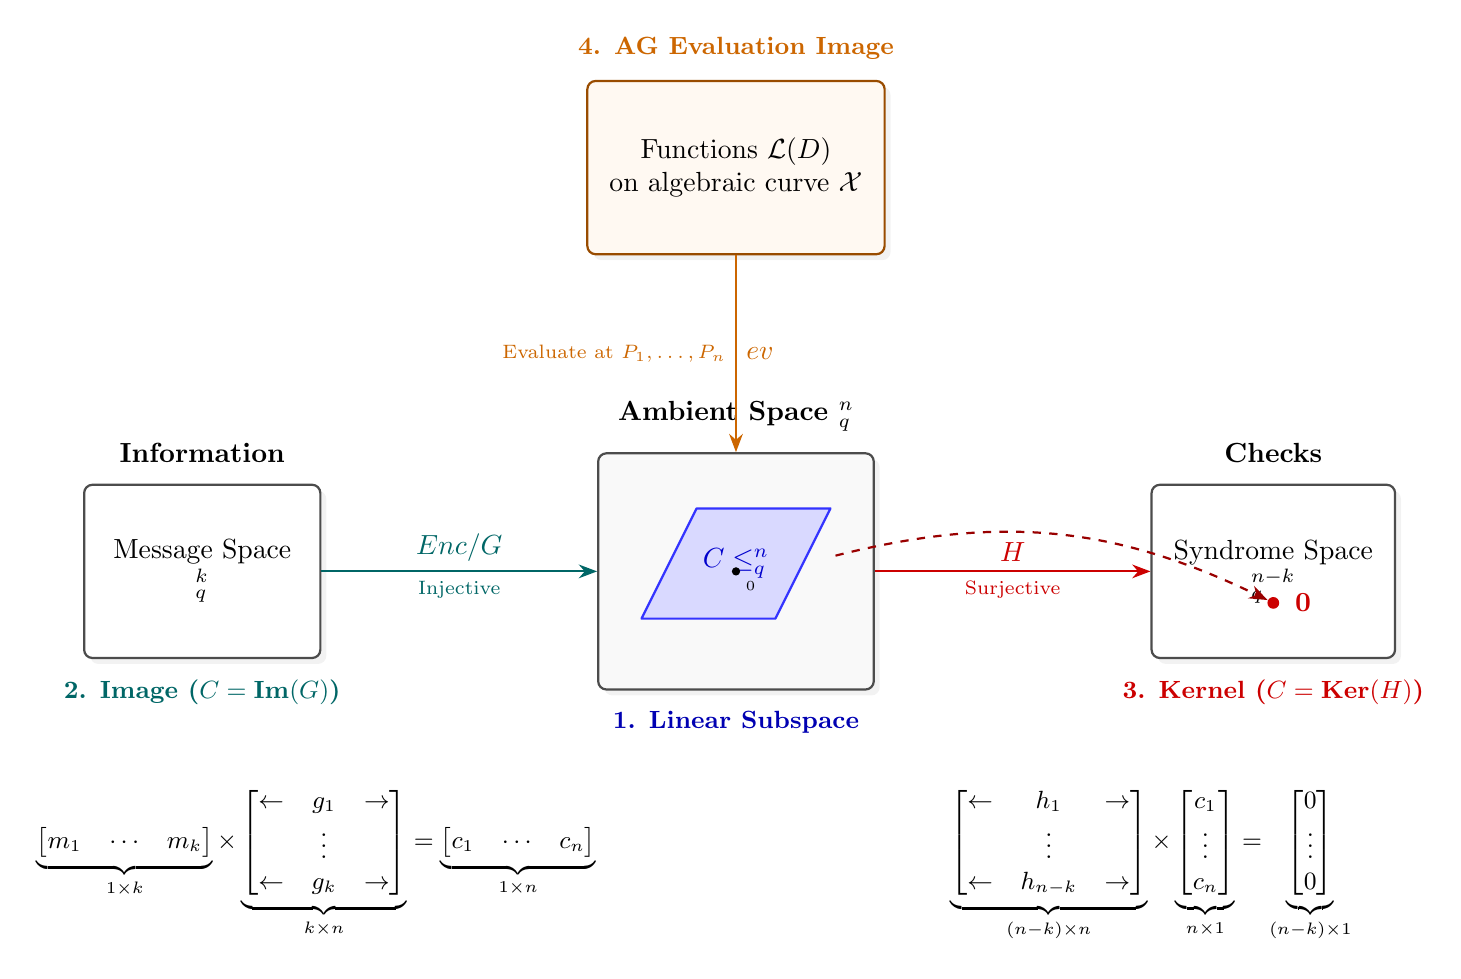
\begin{tikzpicture}[
		>=Stealth,
		% Define box styles for the vector spaces
		spacebox/.style={
			draw=black!70, fill=white, thick, rounded corners=3pt, 
			inner sep=8pt, align=center, minimum height=2.2cm, minimum width=3cm,
			drop shadow={opacity=0.1}
		},
		% Define styles for the matrix equations
		matstyle/.style={
			font=\small, align=center
		}
		]
		
		% ==========================================
		% 1. AMBIENT SPACE & SUBSPACE (Center)
		% ==========================================
		\node[spacebox, fill=gray!5, minimum height=3cm, minimum width=3.5cm] (ambient) at (0,0) {};
		
		% Draw a stylized 3D plane for the linear subspace inside the ambient space box
		\draw[thick, fill=blue!15, draw=blue!80, join=round] 
		(-1.2,-0.6) -- (0.5,-0.6) -- (1.2,0.8) -- (-0.5,0.8) -- cycle;
		\node[font=\bfseries, text=blue!80!black] at (0,0.1) {$C \leq \F_q^n$};
		\fill[black] (0,0) circle (1.5pt) node[below right, font=\tiny] {$0$};
		
		\node[above=4pt of ambient, font=\bfseries] {Ambient Space $\F_q^n$};
		\node[below=4pt of ambient, font=\small\bfseries, text=blue!70!black] {1. Linear Subspace};
		
		% ==========================================
		% 2. MESSAGE SPACE & ENCODING (Left)
		% ==========================================
		\node[spacebox, left=3.5cm of ambient] (msg) {Message Space \\ $\F_q^k$};
		
		% Mapping arrow
		\draw[->, thick, teal!80!black] (msg.east) -- (ambient.west) 
		node[midway, above, font=\bfseries] {$Enc / G$} 
		node[midway, below, font=\scriptsize] {Injective};
		
		\node[above=4pt of msg, font=\bfseries] {Information};
		\node[below=4pt of msg, font=\small\bfseries, text=teal!80!black] {2. Image ($C = \text{Im}(G)$)};
		
		% Matrix visual for Encoding (c = mG)
		\node[matstyle, below=1.5cm of msg, xshift=1.5cm] (encmat) {
			$\underbrace{\begin{bmatrix} m_1 & \cdots & m_k \end{bmatrix}}_{1 \times k}
			\times
			\underbrace{\begin{bmatrix} \leftarrow & g_1 & \rightarrow \\ & \vdots & \\ \leftarrow & g_k & \rightarrow \end{bmatrix}}_{k \times n}
			=
			\underbrace{\begin{bmatrix} c_1 & \cdots & c_n \end{bmatrix}}_{1 \times n}$
		};
		
		% ==========================================
		% 3. SYNDROME SPACE & PARITY CHECK (Right)
		% ==========================================
		\node[spacebox, right=3.5cm of ambient] (synd) {Syndrome Space \\ $\F_q^{n-k}$};
		
		% Mapping arrow
		\draw[->, thick, red!80!black] (ambient.east) -- (synd.west) 
		node[midway, above, font=\bfseries] {$H$} 
		node[midway, below, font=\scriptsize] {Surjective};
		
		\node[above=4pt of synd, font=\bfseries] {Checks};
		\node[below=4pt of synd, font=\small\bfseries, text=red!80!black] {3. Kernel ($C = \text{Ker}(H)$)};
		
		% Vector mapping visual to 0 inside Syndrome space
		\node[circle, fill=red!80!black, inner sep=1.5pt] (zero) at ($(synd) + (0,-0.4)$) {};
		\node[right=2pt of zero, text=red!80!black, font=\bfseries] {$\mathbf{0}$};
		
		% Draw dashed arrow showing the whole plane mapping to zero
		\draw[->, dashed, thick, red!60!black] ($(ambient.east) + (-0.5, 0.2)$) to[bend left=20] (zero);
		
		% Matrix visual for Parity Check (Hc^T = 0)
		\node[matstyle, below=1.5cm of synd, xshift=-1.5cm] (chkmat) {
			$\underbrace{\begin{bmatrix} \leftarrow & h_1 & \rightarrow \\ & \vdots & \\ \leftarrow & h_{n-k} & \rightarrow \end{bmatrix}}_{(n-k) \times n}
			\times
			\underbrace{\begin{bmatrix} c_1 \\ \vdots \\ c_n \end{bmatrix}}_{n \times 1}
			=
			\underbrace{\begin{bmatrix} 0 \\ \vdots \\ 0 \end{bmatrix}}_{(n-k) \times 1}$
		};
		
		% ==========================================
		% 4. AG VIEWPOINT (Top)
		% ==========================================
		\node[spacebox, fill=orange!5, draw=orange!60!black, above=2.5cm of ambient] (ag) {
			Functions $\mathcal{L}(D)$ \\ on algebraic curve $\mathcal{X}$
		};
		
		% Mapping arrow
		\draw[->, thick, orange!80!black] (ag.south) -- (ambient.north) 
		node[midway, right, font=\bfseries] {$ev$} 
		node[midway, left, font=\scriptsize] {Evaluate at $P_1, \dots, P_n$};
		
		\node[above=4pt of ag, font=\small\bfseries, text=orange!80!black] {4. AG Evaluation Image};
		
	\end{tikzpicture}
	
\end{document}